\documentclass[12pt]{article}

\usepackage{amsfonts}
\usepackage{enumitem}
\usepackage{graphicx}
\usepackage{amsmath}
\usepackage{mathrsfs}

\begin{document}
\begin{center}
\Large{\textbf{ECON 634 Problem Set 3}}\\[3mm]
\large{{Mingyang Li}}\\[1mm]
\today
\end{center}
\vfill

\begin{enumerate}
\item The recursive problem is 
$$\max_{\{c_t\}_{t=0}^\infty}\mathbb{E}_0\left[\sum_{t=0}^\infty\beta^t u(c_t)\right]$$
$$s.t.\ c_t+q_ta_{t+1}=y(s_t)+a_t$$
$$a_{t+1}\in\Gamma(s_t,a_t)$$
$$a_{t+1}\geq\underbar{$a$},\ \forall t,\ \text{and}\ a_0\ \text{given.}$$
The functional equation of the dynamic programming problem is
$$V(s,a)=\max_{a'\in\Gamma(s,a)} \left\{\frac{[y(s)+a-qa']^{(1-\sigma)}}{1-\sigma}+\beta\mathbb{E}_{s'|s}V(s',a')\right\}$$
where $s$ and $a$ are the state variables and $s'$ and $a'$ are the control variables.\\
The state space is the combination of the possible states of asset $$\mathscr{A}=\{a_1,a_2,...,a_n\}$$ and the possible states of employment $$\mathscr{S}=\{e,u\}.$$
The constraint correspondence is $$\Gamma(a,s)=\left\{a':a'\geq0,\ a'\leq\frac{y(s)+a}{q}\right\}.$$
\\[10mm]
\vfill
\item The market clearing bond price is $q^{ss} = 0.9943$. Therefore, the risk-free interest rate in the economy in the steady state is $\frac{1}{q^{ss}} = 1.0057$.\\The plot of value functions is following:
\begin{center}
  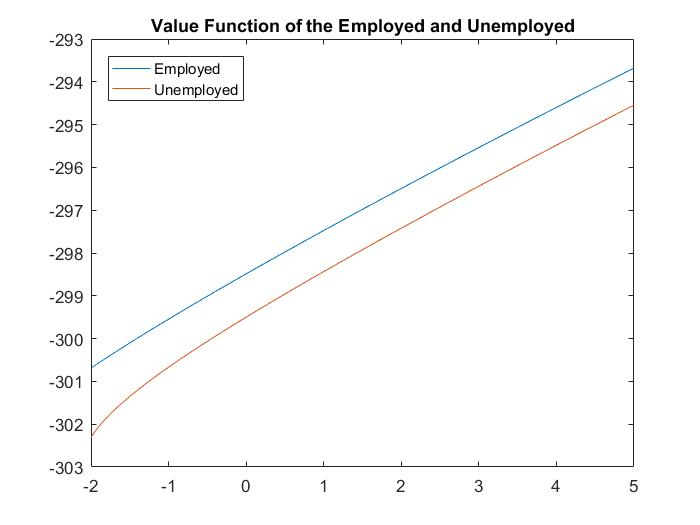
\includegraphics[width=130mm]{ValueFunction.jpg}
\end{center}
\pagebreak
\item The plots of Lorenz Curves are following:
\begin{center}
  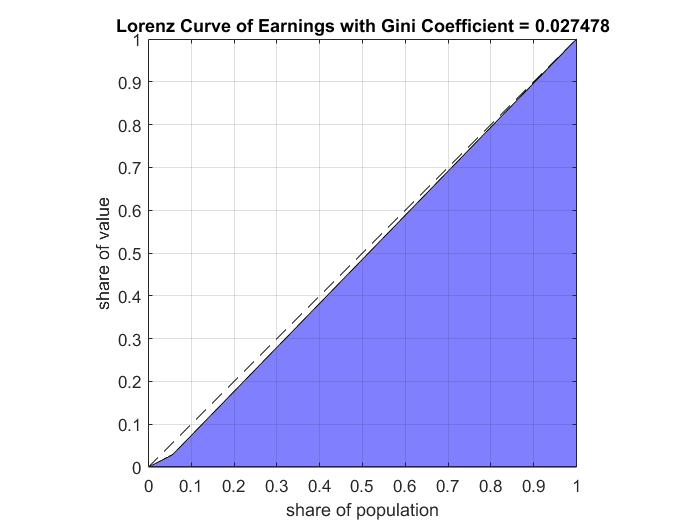
\includegraphics[width=111.11mm]{LorenzCurveofEarnings.jpg}
\end{center}
\begin{center}
  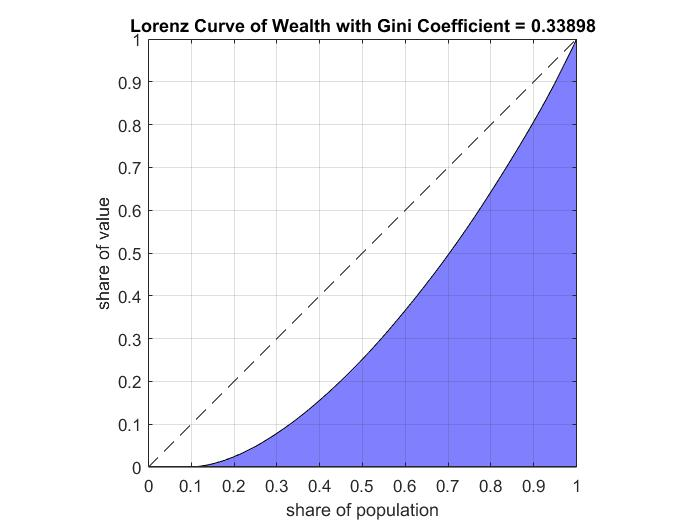
\includegraphics[width=111.11mm]{LorenzCurveofWealth.jpg}
\end{center}

\end{enumerate}

\end{document}